A \gls{kdf} is a cryptographic algorithm that generates keying material that cryptographic algorithms can use. The function requires two sorts of input: a secret value, such as a key or a password, and other data. The core of a KDF is often built using a pseudorandom function, such as Keyed cryptographic hash functions. A key derivation function iterates an n-bit pseudorandom function and concatenates the outputs until L bits of keying material are generated. Each output receives a distinct value with each cycle, thus if one key is compromised, the risk is isolated to that key while preceding keys remain secure. \gls{nist} proposed recommended techniques to use pseudorandom-based \glspl{kdf} in \cite{chen2008recommendation}. 
\begin{figure}[hptb]
	\centering
	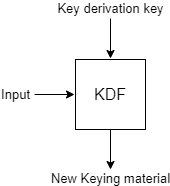
\includegraphics[scale=0.65]{Images/kdf.png}
	\caption{Key derivation function.}
	\label{fig:kdf}
\end{figure}